% This must be in the first 5 lines to tell arXiv to use pdfLaTeX, which is strongly recommended.
% \pdfoutput=1
% In particular, the hyperref package requires pdfLaTeX in order to break URLs across lines.

\documentclass[11pt]{article}

% Remove the "review" option to generate the final version.
% \usepackage[review]{ACL2023}
\usepackage[]{ACL2023}

% Standard package includes
\usepackage{times}
\usepackage{latexsym}

% For proper rendering and hyphenation of words containing Latin characters (including in bib files)
\usepackage[T1]{fontenc}
% For Vietnamese characters
% \usepackage[T5]{fontenc}
% See https://www.latex-project.org/help/documentation/encguide.pdf for other character sets

% This assumes your files are encoded as UTF8
\usepackage[utf8]{inputenc}

% This is not strictly necessary, and may be commented out.
% However, it will improve the layout of the manuscript,
% and will typically save some space.
\usepackage{microtype}

% This is also not strictly necessary, and may be commented out.
% However, it will improve the aesthetics of text in
% the typewriter font.
\usepackage{inconsolata}

\usepackage{booktabs}
\usepackage{tikz}
\usepackage[autostyle, english=american]{csquotes}
\MakeOuterQuote{"}

\usepackage{amsmath}
\DeclareMathOperator{\PPL}{PPL}
\DeclareMathOperator{\PPPL}{PPPL}

% If the title and author information does not fit in the area allocated, uncomment the following
%
%\setlength\titlebox{<dim>}
%
% and set <dim> to something 5cm or larger.

\title{Perplexity as a Measure for Temporal Common Sense in Pre-Trained Language Models}

% Author information can be set in various styles:
% For several authors from the same institution:
% \author{Author 1 \and ... \and Author n \\
%         Address line \\ ... \\ Address line}
% if the names do not fit well on one line use
%         Author 1 \\ {\bf Author 2} \\ ... \\ {\bf Author n} \\
% For authors from different institutions:
% \author{Author 1 \\ Address line \\  ... \\ Address line
%         \And  ... \And
%         Author n \\ Address line \\ ... \\ Address line}
% To start a seperate ``row'' of authors use \AND, as in
% \author{Author 1 \\ Address line \\  ... \\ Address line
%         \AND
%         Author 2 \\ Address line \\ ... \\ Address line \And
%         Author 3 \\ Address line \\ ... \\ Address line}

% \author{First Author \\
%   Affiliation / Address line 1 \\
%   Affiliation / Address line 2 \\
%   Affiliation / Address line 3 \\
%   \texttt{email@domain} \\\And
%   Second Author \\
%   Affiliation / Address line 1 \\
%   Affiliation / Address line 2 \\
%   Affiliation / Address line 3 \\
%   \texttt{email@domain} \\}
 
\author{Tai Mai \\
  \texttt{mai@cl.uni-heidelberg.de} \\
  \\}

\begin{document}
\maketitle
\begin{abstract}
This document is a supplement to the general instructions for *ACL authors. It contains instructions for using the \LaTeX{} style file for ACL 2023.
The document itself conforms to its own specifications, and is, therefore, an example of what your manuscript should look like.
These instructions should be used both for papers submitted for review and for final versions of accepted papers.
\end{abstract}

\section{Introduction}

Language models nowadays see an ever increasing amount of data during their pre-training. For example, GPT-2 \citep{gpt2} was trained on 40 GB of text scraped from the web. RoBERTa \citep{roberta} was trained on over 160 GB of text, comprised of books, Wikipedia and news articles, as well as text scraped from the web. Llama-3.1 \citep{llama3} is a very recent model that was trained on over 15 trillion tokens of publicly available online data. While these figures aren't directly comparable, they speak to the vast amounts data that are used to pre-train a language model. Language models are typically pre-trained in an unsupervised manner. For example, causal language models such as GPT-2 \citep{gpt2} and Llama-3.1 \citep{llama3} generate text by predicting tokens one by one, each conditioned on the preceding tokens. Their objective is to correctly model their training data by maximizing the likelihood of token sequences that are present in the training data. On the other hand, masked language models such as RoBERTa \citep{roberta} are trained on another unsupervised task known as masked language modeling. In contrast to causal language modeling, masked language modeling is the process of randomly masking tokens in a training sentence and tasking the language model with reconstructing the original sentence based on the context surrounding the masked token. Pre-training a language model is designed to enable it to form an intuition for the language such that the resulting foundation model's intuition can be built upon in different downstream tasks such as classification. This process of specializing a language model for a specific downstream task is called fine-tuning and often entails adding and training a few additional neural layers --- commonly called a task head --- to the pre-trained model to make it compatible with the desired downstream task. Besides obtaining an intuition for the language, pre-trained language models have also been shown to be able to form a semblance of factual common sense through pre-training \citet{zhou2020evaluating}. However, testing a pre-trained language model for common sense in, say, temporal relations can be tricky. For example, employing a language model to classify the relation between two events in time is, in its most straight-forward form, a classification task that would most commonly require fine-tuning a classification head on top of the pre-trained model. Querying a model after fine-tuning, however, makes it impossible to say whether its understanding of time was obtained during pre-training or as a result of fine-tuning. To isolate the effects of pre-training alone, this kind of evaluation has to be done on the foundation model directly, without any further training.

This project attempts an approach to investigate the amount of temporal common sense that different pre-trained foundation language models obtain through pre-training. In lieu of fine-tuning the model for a classification task, the foundation model's perplexity metric is chosen as a proxy for how natural it judges a particular sentence. The results show that perplexity is likely not a good measure to correlate with temporal common sense.

\section{Methods} % (fold)
\label{sec:Methods}

\subsection{Perplexity metrics}
\label{sec:ppl}
Perplexity in language models can be interpreted as a measure of how likely a language model thinks a token sequence is. The higher the perplexity metric is for a particular sequence, the more "surprised" the language model is to see that sequence. Perplexity is most commonly used for causal language modeling (CLM) and is defined as follows\footnote{\url{https://huggingface.co/docs/transformers/en/perplexity}}
\begin{equation}
  \PPL(X) = \exp \left\{ - \frac{1}{t} \sum^t_i \log p_\text{CLM} (x_i | x_{<i}) \right\},
  \label{eq:ppl}
\end{equation}
where $X$ denotes the token sequence of tokens $x$, $t$ is the number of tokens in the sequence, and $p_\theta(x_i | x_{<i})$ represents the probability of token $x_i$ at position $i$, given all the previous tokens $x_{<i}$. Therefore, this definition of perplexity is very specific to causal language modeling and cannot be directly applied to masked language modeling.

To obtain an analogous metric for masked language modeling (MLM), \citet{pppl} propose a pseudo-perplexity metric, defined as follows:
\begin{equation}
  \PPPL(X) := \exp \left\{ - \frac{1}{t} \sum^t_i \log p_\text{MLM} (x_i | X_{\backslash x_i}) \right\}.
  \label{eq:pppl}
\end{equation}
The only difference to Equation~\ref{eq:ppl} is in the context on which the token $x_i$ is conditioned. In causal language modeling, the choice of token $x_i$ at position $i$ is conditioned on all tokens to the left of position $i$. Future tokens cannot be taken into account in causal language modeling, therefore the context is unilateral. In masked language modeling, however, tokens in the sequence are chosen and masked at random. To reconstruct a masked token $x_i$, language models are provided with all other unmasked tokens in the sequence, both before and after position $i$. Therefore, the context in masked language modeling is bilateral.

These metrics are chosen to gauge how natural a language model thinks a sequence is, specifically in the case of temporal relations described in the following section.

\subsection{Allen's Interval Algebra}
\label{sec:allen}
\citet{allen} proposes a system of relating two events $e_1$ and $e_2$ to each other in time via a set of basic temporal relations. This set can be boiled down to the following seven relations:

\begin{itemize}
  \item \textit{before}$(e_1, e_2)$: $e_1$ starts and ends before $e_2$ starts
  \item \textit{meets}$(e_1, e_2)$: $e_1$ starts before $e_2$ and $e_2$ starts when $e_1$ ends
  \item \textit{overlaps}$(e_1, e_2)$: $e_1$ starts before $e_2$ and $e_1$ ends between the start and end of $e_2$
  \item \textit{starts}$(e_1, e_2)$: $e_1$ starts at the same time as $e_2$ and $e_1$ ends before $e_2$
  \item \textit{during}$(e_1, e_2)$: $e_1$ starts after $e_2$ and $e_1$ ends before $e_2$
  \item \textit{finishes}$(e_1, e_2)$: $e_1$ starts after $e_2$ and $e_1$ ends at the same time as $e_2$
  \item \textit{equals}$(e_1, e_2)$: $e_1$ starts and ends at the same time as $e_2$
\end{itemize}

The complete set proposed by \citet{allen} also contains inverses of the previous relations. However, these inverses can also be modeled by the seven relations above by simply swapping the positions of the events as arguments to the relations, i.e.~\textit{after}$(e_1, e_2)$ is equivalent to \textit{before}$(e_2, e_1)$. Therefore, this project will only consider the seven relations mentioned above. These relations can then also be verbalized into natural language. For example, one possible verbalization of the relation \textit{before} could be "$e_1$ \textit{happens before} $e_2$." An event tuple such as $\langle \text{birth}, \text{death} \rangle$ can then be connected and verbalized as \textit{"Birth happens before death."} The objective of this project is to investigate how well the perplexity values of these verbalizations correlate with temporal common sense. Specifically, the first hypothesis investigated in this project is that a verbalization that reflects temporal common sense, such as \textit{"Birth happens before death,"} should receive a lower perplexity score than one that does not reflect temporal common sense, such as \textit{"Birth happens during death."}

\subsection{Conceptual neighborhood}

\begin{figure}
  \begin{center}
    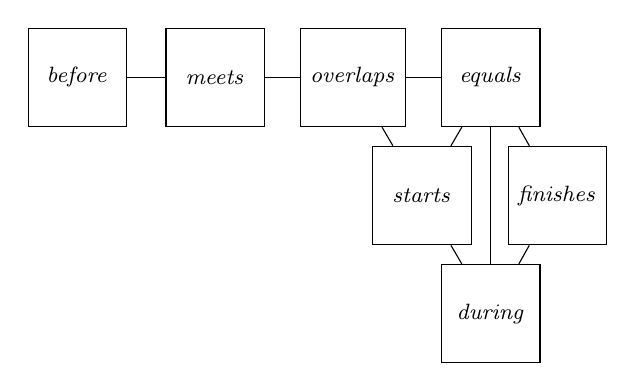
\begin{tikzpicture}[node distance=2cm, every node/.style={draw, minimum size=1.25cm, font=\footnotesize, text centered}]
      % Nodes
      \node (before) at (0, 0) {\textit{before}};
      \node (meets) at (1.75, 0) {\textit{meets}};
      \node (overlaps) at (3.5, 0) {\textit{overlaps}};
      \node (equals) at (5.25, 0) {\textit{equals}};
      \node (during) at (5.25, -3) {\textit{during}};
      \node (starts) at (4.375, -1.5) {\textit{starts}};
      \node (finishes) at (6.095, -1.5) {\textit{finishes}};

      % Edges
      \draw (before) -- (meets);
      \draw (meets) -- (overlaps);
      \draw (overlaps) -- (equals);
      \draw (overlaps) -- (starts);
      \draw (equals) -- (starts);
      \draw (equals) -- (during);
      \draw (equals) -- (finishes);
      \draw (starts) -- (during);
      \draw (finishes) -- (during);
    \end{tikzpicture}
  \end{center}
  \caption{Conceptual neighborhood according to \citet{freksa}, excluding the inverse relations.}
  \label{fig:conceptual_neighborhood}
\end{figure}


\citet{freksa} arranges the relations proposed by \citet{allen} in an undirected graph structure to encode how closely two relations are related to each other. Figure~\ref{fig:conceptual_neighborhood} shows this graph after excluding the inverse relations. With this graph structure in mind, this project attempts to investigate whether the perplexity scores correlate with the conceptual distance in graph hops. As an example, the relations \textit{before} and \textit{during} are separated by four node hops in the conceptual neighborhood graph. As mentioned in Section~\ref{sec:allen}, we hypothesize that an atypical verbalization, such as \textit{"Birth happens during death,"} should receive a higher perplexity score than a common sense verbalization, such as \textit{"Birth happens before death."} Therefore, the second hypothesis investigated in this project is that this change in perplexity correlates with the degrees of separation between the two relations.

\section{Data}
To test these two hypotheses, a simple dataset has been constructed by utilizing Claude 3.5 Sonnet\footnote{\url{https://www.anthropic.com/news/claude-3-5-sonnet}} and then been curated by hand. For each of the seven temporal relations, a set of 20 event tuples are gathered which are examples of the temporal relation at hand. For the relation \textit{before}, one of the examples collected is the tuple $\langle \text{birth}, \text{death}\rangle$.
Furthermore, for each of the relations, a set of ten possible verbalizations is gathered, with \texttt{\{event1\}} and \texttt{\{event2\}} as placeholders for respective temporal events, for example \textit{"\texttt{\{event1\}} happens before \texttt{\{event2\}}."}
Every event tuple is then placed into every verbalization of every relation, yielding a total dataset size of $20 \cdot 10 \cdot 7 = 140$ verbalized examples.

Before Claude 3.5 Sonnet was released, GPT 3.5 and GPT4o\footnote{\url{https://chatgpt.com}} were also considered for this task. However, upon manual inspection of the generated data, these models did not prove to be able to come up with (enough) correct and/or diverse examples and were subsequently dropped in favor of Claude 3.5 Sonnet, which required a lot less manual intervention. The conversation prompts used to generate this dataset can be seen in Appendix~\ref{sec:prompts}.

\section{Evaluation} % (fold)
\label{sec:Evaluation}
\subsection{Correlation analysis}
\begin{table*}
  \centering
  \begin{tabular}{l c c c}
    \toprule
    Model & $r$ & $\rho$ & $\tau$ \\
    \midrule
    % \arrayrulecolor{black! 30}\midrule  % needs \usepackage[table]{xcolor}
    GPT-2 & $0.0537$ & $0.0654$ & $0.0477$ \\
    GPT-2 (normalized) & $0.0407$ & $0.0608$ & $0.0444$ \\
    RoBERTa-base & $0.0266$ & $0.0906$ & $0.0661$ \\
    RoBERTa-base (normalized) & $0.0231$ & $0.0876$ & $0.0638$ \\
    Llama-3.1 8B & $0.0483$ & $0.1230$ & $0.0901$ \\
    Llama-3.1 8B (normalized) & $0.0571$ & $0.1212$ & $0.0884$ \\
    \bottomrule
    % \arrayrulecolor{black}\bottomrule % needs \usepackage[table]{xcolor}
  \end{tabular}
  \caption{Pearson's $r$, Spearman's $\rho$, and Kendall's $\tau$ correlation coefficients between \emph{raw perplexity values} and graph hops.}
  \label{raw_correlations}
\end{table*}

\begin{table*}
  \centering
  \begin{tabular}{l c c c}
    \toprule
    Model & $r$ & $\rho$ & $\tau$ \\
    \midrule
    % \arrayrulecolor{black! 30}\midrule  % needs \usepackage[table]{xcolor}
    GPT-2 & $0.0319$ & $-0.0968$ & $-0.0698$ \\
    GPT-2 (normalized) & $0.0087$ & $-0.0419$ & $-0.0304$ \\
    RoBERTa-base & $0.0106$ & $-0.0484$ & $-0.0342$ \\
    RoBERTa-base (normalized) & $0.0094$ & $-0.0126$ & $-0.0087$ \\
    Llama-3.1 8B & $0.0242$ & $-0.0665$ & $-0.0469$ \\
    Llama-3.1 8B (normalized) & $0.0278$ & $-0.0224$ & $-0.0148$ \\
    \bottomrule
    % \arrayrulecolor{black}\bottomrule % needs \usepackage[table]{xcolor}
  \end{tabular}
  \caption{Pearson's $r$, Spearman's $\rho$, and Kendall's $\tau$ correlation coefficients between \emph{perplexity deltas} and graph hops.}
  \label{delta_correlations}
\end{table*}
% section Evaluation (end)
%
% Entries for the entire Anthology, followed by custom entries
% \bibliography{anthology,custom}
\bibliography{references}
\bibliographystyle{acl_natbib}

\appendix
\onecolumn

\section{Claude 3.5 Sonnet Prompting for the Dataset Generation}
\label{sec:prompts}
\begin{enumerate}
  \item "What are the relations in James Allen's interval calculus?"
    \begin{itemize}
      \item James Allen's Interval Calculus, introduced in 1983, defines 13 basic relations between time intervals. These relations describe all possible ways two time intervals can be related to each other. Here's a concise list of the 13 relations:
        \begin{enumerate}
          \item Before (precedes)
          \item Meets
          \item Overlaps
          \item Starts
          \item During
          \item Finishes
          \item Equals
          \item Finished-by
          \item Contains
          \item Started-by
          \item Overlapped-by
          \item Met-by
          \item After (follows)
        \end{enumerate}
These relations are mutually exclusive and exhaustive, meaning any two time intervals must be related by exactly one of these relations. Each relation also has an inverse (e.g., "before" is the inverse of "after"), which is why there are 13 relations instead of 7.
Would you like me to elaborate on any specific relation or provide examples of how these relations are used in temporal reasoning?
    \end{itemize}
  \item "Give me the relations without the inverses"
    \begin{itemize}
      \item Certainly. If we consider only the base relations without their inverses, we can reduce James Allen's Interval Calculus to 7 fundamental relations. Here they are:
        \begin{enumerate}
          \item Before
          \item Meets
          \item Overlaps
          \item Starts
          \item During
          \item Finishes
          \item Equals
        \end{enumerate}
These 7 relations form the core of Allen's Interval Calculus. The other 6 relations in the full set of 13 are inverses of these (except for "Equals," which is its own inverse).
Would you like me to explain how these relations are defined or provide examples of their use in temporal reasoning?
    \end{itemize}
  \item "Please define each of these seven relations in Allen's Interval Calculus."
    \begin{itemize}
      \item Certainly. I'll define each of the seven base relations in Allen's Interval Calculus. Let's consider two time intervals, A and B:
        \begin{enumerate}
          \item Before (A before B):
            Interval A ends before interval B starts. There is a gap between A and B.
          \item Meets (A meets B):
            The end point of interval A is exactly the start point of interval B. There is no gap between them.
          \item Overlaps (A overlaps B):
            Interval A starts before B, and they overlap for some duration. A ends sometime after B starts but before B ends.
          \item Starts (A starts B):
            Both intervals start at the same point, but A ends before B ends.
          \item During (A during B):
            Interval A starts after B starts and ends before B ends. A is completely contained within B.
          \item Finishes (A finishes B):
            Both intervals end at the same point, but A starts after B starts.
          \item Equals (A equals B):
            Both intervals start and end at the same points. They are identical in duration and position.
        \end{enumerate}
        These definitions assume that intervals are non-zero in duration and have distinct start and end points. Each relation (except "Equals") has an inverse relation in the full set of 13 relations.
        Would you like me to provide visual representations or examples of these relations?
    \end{itemize}
  \item "For each of these relations, give me 10 commonsense examples of temporal events or periods . They should always and universally be true. Don't use examples that are just "often" or "sometimes" the case. Make sure not to confuse "before" with "meets". Also, don't confuse "finishes" with "after". For "meets", don't mention the point in time where they meet. Format the examples in JSON like this:
    \{ "before": [ \{ "event1": "breakfast", "event2": "lunch", "example": "breakfast happens before lunch." \}, \{ "event1": ..., ... \}, ] ...\}"
    \begin{itemize}
      \item I understand your request. I'll provide 10 commonsense examples for each of the seven relations in Allen's Interval Calculus, ensuring they are always and universally true. I'll format them in JSON as requested, being careful to distinguish between "before" and "meets", and between "finishes" and "after". Here's the JSON with the examples:
        [...]
  I've created a JSON structure with 10 examples for each of the seven relations in Allen's Interval Calculus. These examples are designed to be universally true and not just "often" or "sometimes" the case. I've been careful to distinguish between "before" and "meets", as well as between "finishes" and "after". For the "meets" relation, I've avoided mentioning the specific point in time where the events meet.
  Each relation has its own array of examples, and each example is structured with "event1", "event2", and an "example" sentence describing the relation between the events.
  Is there anything you'd like me to clarify or expand upon regarding these examples or Allen's Interval Calculus?
    \end{itemize}
  \item "Please do the same thing again and create 10 new examples for each relation. Do not repeat the ones you've created so far. Take care that the "equals" relation needs to be about temporal periods only."
    \begin{itemize}
      \item Certainly, I'll create 10 new examples for each relation, ensuring they are distinct from the previous set and that the "equals" relation focuses solely on temporal periods. I'll maintain the same JSON structure and adhere to the guidelines you've provided.
        [...]
I've created a new set of 10 examples for each of the seven relations in Allen's Interval Calculus. These examples are distinct from the previous set and adhere to the guidelines you provided. For the "equals" relation, I've ensured that all examples focus solely on temporal periods.
Each relation is represented by an array of examples, with each example containing "event1", "event2", and an "example" sentence describing the relation between the events.
Is there anything you'd like me to clarify or expand upon regarding these new examples or Allen's Interval Calculus?
    \end{itemize}
  \item "For each of the relations, generate me a list of possible verbalizations by using placeholders for the two events. Format it as JSON like this: \{ "before": [ "\{event1\} happens before \{event2\}" ... ], ... \}"
    \begin{itemize}
      \item Certainly! I'll create a list of possible verbalizations for each of Allen's Interval Calculus relations, using placeholders for the two events. I'll format this as JSON as you've requested.
        [...]
        I've created a JSON structure with 10 possible verbalizations for each of the seven relations in Allen's Interval Calculus. Each verbalization uses placeholders {event1} and {event2} to represent the two events being related.
These verbalizations provide various ways to express each temporal relationship, ranging from simple and direct statements to more elaborate descriptions. They can be useful for natural language processing tasks, generating descriptions of temporal relationships, or for explaining these concepts in different contexts.
Is there anything you'd like me to clarify or expand upon regarding these verbalizations or Allen's Interval Calculus?
    \end{itemize}
\end{enumerate}


\end{document}
